\documentclass{beamer}
\usepackage[style=numeric-comp, backend=biber]{biblatex}
\usepackage{lmodern}
\usepackage{amsmath}
\usepackage{mathtools}
\usepackage[utf8]{inputenc}

\graphicspath{{./Figures/}}
%smaller footnotes, adapted from http://tex.stackexchange.com/a/146021
\setbeamerfont{footnote}{size=\fontsize{7pt}{0pt}}

%footnote spacing avoids navigation / margins, adapted from http://tex.stackexchange.com/a/44231
\addtobeamertemplate{footnote}{\vspace{-6pt}\advance\hsize-0.5cm}{\vspace{6pt}}
\makeatletter
% Alternative A: footnote rule
\renewcommand*{\footnoterule}{\kern -3pt \hrule \@width 2in \kern 8.6pt}
% Alternative B: no footnote rule
% \renewcommand*{\footnoterule}{\kern 6pt}
\makeatother

\bibliography{lit_review.bib}

%opening
\title{SIMT\slash SIMD computation on CPUs and Co-processors: A Literature Review}
\author{Nick Curtis}
\institute{University of Connecticut}
\date{\today}

\begin{document}

\maketitle

\begin{frame}
\frametitle{Chemical Kinetic Simulations are \textbf{Critical}}
In order to meet increasingly stringent emissions and efficiency requirements, designers of combustion devices have turned to \textbf{new technologies} and \textbf{new fuels}
\begin{itemize}
 \item Novel combustion regimes such as low-temperature combustion are often controlled by chemical processes, rather than directly controllable physical processes as in current technology
 \item Further, developed solutions must be flexible to accommodate a variety of next generation fuels
\end{itemize}
Computationally guided combustion design has played an important role in development of these new technologies, however use of realistic chemical modeling (as required for predictive reacting-flow simulations) is prohibitively expensive for most practical systems. 
\end{frame}

\begin{frame}
 \frametitle{Chemical Kinetic Integration is \textbf{Expensive}}
 The size of chemical kinetic models for fuels relevant transportation and energy generation may consist of hundreds to thousands of chemical species, with potentially tens of thousands of reactions
 \begin{itemize}
  \item e.g., for gasoline \footfullcite{Mehl:2011cn} and jet fuel\footfullcite{Naik2011434}
 \end{itemize}
 Commonly used implicit integration integration techniques scales poorly with increasing model size.
 \begin{itemize}
  \item These methods require repeated evaluation and factorization of the chemical kinetic Jacobian.
  \item Naive implementations of these operations scale \textbf{quadratically} and \textbf{cubically} with the number of species in a model, respectively\footfullcite{Lu:2009gh}.
 \end{itemize}
\end{frame}

\begin{frame}
 \frametitle{Strategies for cost reduction}
 A few major strategies exist to accelerate chemical kinetic integration:
 \begin{itemize}
  \item \textbf{Model reduction}, a host of techniques to reduce the size of the system being solved while maintaining accurate chemical kinetics (as compared to the full model)
  \item \textbf{Improved integration techniques}, development of new integration algorithms specifically for chemical kinetics, e.g. hybrid implicit\slash explicit integrators, tabulation techniques, analytical Jacobian codes, and on-the-fly stiffness removal
  \item \textbf{Solver vectorization}, reformulation of solvers for efficient single-instruction, multiple-data (SIMD) execution both on specialized hardware---e.g. graphics processing units (GPUs)---and modern central processing units (CPUs)
  \item \textbf{High performance computing techniques}, stiffness-based load balancing, scaling for high performance clusters
 \end{itemize}
 We will focus on \textbf{vectorization} and \textbf{high performance computing}.
\end{frame}

\begin{frame}
 \frametitle{Single Instruction, Multiple Data Processing}
 \begin{columns}
 
 \begin{column}{0.6\textwidth}
  \textbf{Single Instruction, Multiple Data (SIMD)} processing is a vector processing paradigm that allows processing elements (PE)---e.g a CPU core---to execute the same instruction concurrently on different data.
  \begin{itemize}
    \item Each vector unit contains multiple processing units (PUs), which are called a \textbf{lane}
    \item Typically one thread resides on each PE, each issuing SIMD vector instructions
    \begin{itemize}
     \item It is possible to have multiple threads per PE, but SIMD instructions between threads do not interact
    \end{itemize}
  \end{itemize}
 \end{column}
 \begin{column}{0.4\textwidth}
  \begin{figure}
    \centering
    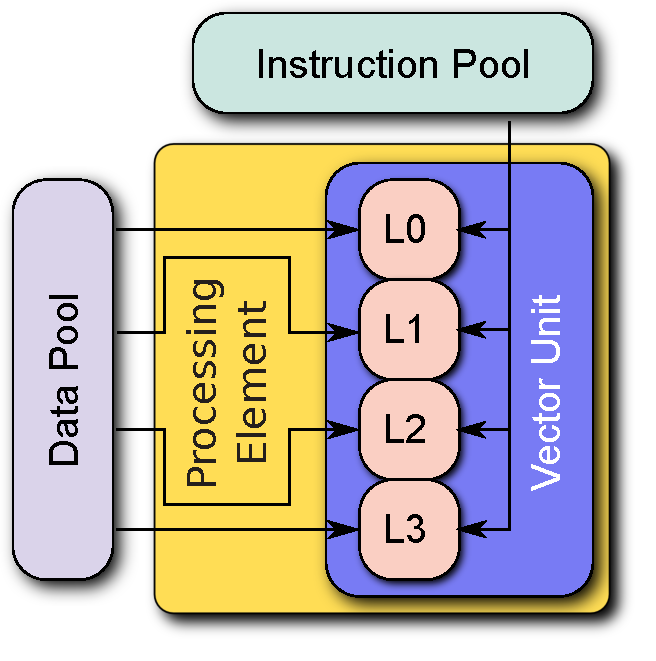
\includegraphics[width=\columnwidth]{SIMD.pdf}
    \caption{Schematic of SIMD processing.  Adapted from\footnotemark}
  \end{figure}
 \end{column}
 \footnotetext{\fullcite{Simdfig:2016}}
 \end{columns}
\end{frame}

\begin{frame}
 \frametitle{Single Instruction, Multiple Thread Processing}
 \begin{columns}
 \begin{column}{0.6\textwidth}
 \textbf{Single instruction, multiple thread (SIMT)} processing is a related, though separate concept.
 \begin{itemize}
  \item Multiple threads reside on a PE, each with instructions to execute at each step (\textrm{I1}, \textrm{I2} in the example)
  \item All threads that need to execute the same instruction (e.g. \textrm{I1}) execute simultaneously
  \item If some threads need a different instruction (e.g. \textrm{I2}), they must wait and execute their instruction after the other threads
  \item This is known as \textbf{thread divergence}, and is an important performance concern.
 \end{itemize}

  
 \end{column}
 \begin{column}{0.4\textwidth}
  \begin{figure}[r]
    \centering
    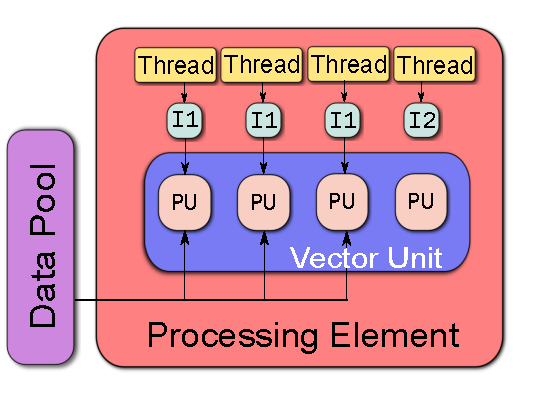
\includegraphics[width=\columnwidth]{SIMT.pdf}
    \caption{Schematic of SIMT processing}
  \end{figure}
 \end{column}
 \end{columns}
\end{frame}

    
\begin{frame}
 \frametitle{Single Instruction, Multiple Data\slash Thread Processing (2)}
 Different levels of parallelism are available:
 \begin{itemize}
  \item Multiple PEs available (e.g. SIMT processing)
  \begin{itemize}
   \item Multiple threads may reside on a single CPU core (\textbf{hyperthreading})
  \end{itemize}
  \item SIMD processing within a PE
 \end{itemize}
\end{frame}

\end{document}
